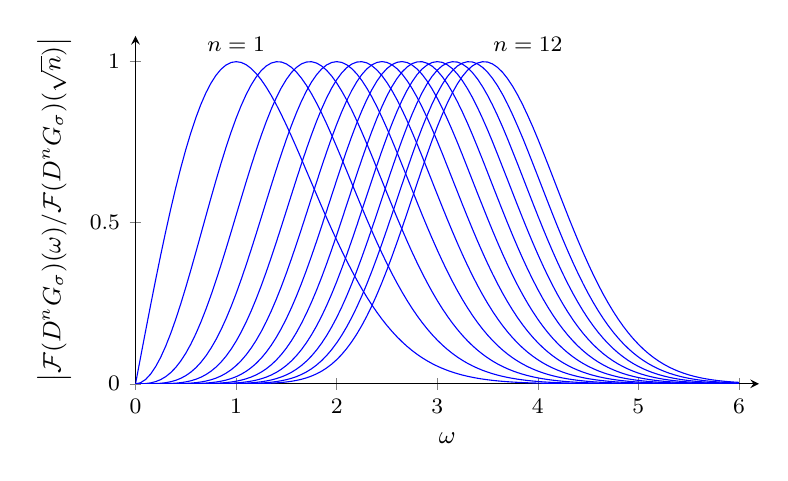
\begin{tikzpicture}
  \begin{axis}[width=9.5cm, height=6cm, axis lines=left,
      xmin=0, xmax=6.2, ymin=0, ymax=1.08,
      xlabel={$\omega$},
      ylabel={$\bigl|\mathcal{F}(D^nG_\sigma)(\omega)/\mathcal{F}(D^nG_\sigma)(\sqrt{n})\bigr|$},
      ylabel style={font=\small}, xlabel style={font=\small},
      ticklabel style={font=\footnotesize},
      domain=0:6, samples=121, no markers]
    \pgfplotsinvokeforeach{1,...,12}{
      \addplot[blue, thin] {(x/sqrt(#1))^(#1)*exp(-(x^2-#1)/2)};
    }
    \node[font=\footnotesize, anchor=south] at (axis cs:1,1.0) {$n=1$};
    \node[font=\footnotesize, anchor=south west] at (axis cs:3.46,1.0) {$n=12$};
  \end{axis}
\end{tikzpicture}
